%
% deeper_insight.tex
% Student Loans
%
% Created by Ed Silkworth on 6/7/19.
% Copyright © 2019 Ed Silkworth. All rights reserved.
%
% All problems detected in this document have been resolved.
% 

\documentclass[12pt,letterpaper,oneside]{article}

% preamble
\usepackage{amsthm, amsmath, mathtools, fancyhdr, cases, cleveref, amssymb, setspace, xcolor, chngcntr, alphalph, graphicx, float}
\usepackage[document]{ragged2e} % left-aligns content
\graphicspath{ {./images/} }
\usepackage{mathptmx} % times new roman font for text and mathematics
\usepackage[normalem]{ulem} % ``normalem'' to prevent underline in algorithm
\usepackage[vlined]{algorithm2e} % no ``end''
\usepackage[left=1.5in, top=1in, right=1in, bottom=1in]{geometry} % left margin of dissertation is 1.5in
\pagestyle{fancy} % enables custom header/footer
\renewcommand{\thispagestyle}[1]{} % prevent changing style
\rhead{} % do not display page number on first page
\lhead{}
% \setcounter{page}{224} % match page number in dissertation
\renewcommand{\headrulewidth}{0pt} % no header underline
\setlength{\topmargin}{-0.2in} % places header page number about 0.75in from top of page; ``\topmargin'' is specifically for header
\setlength{\headheight}{14.5pt} % addresses warning about \headheight being too small
\setlength{\headsep}{0.07in} % places document text about 1in from top of page; essentially a bottom margin for header
\cfoot{} % no footer
\newtheorem{theorem}{Theorem}[section] % [section] provides #.# for theorems
\newtheorem{definition}[theorem]{Definition} % embedding [theorem] provides 1.1, 1.2, 1.3, ... for definitions
\newtheorem{example}{Example}[section]
\def\theexample{\arabic{section}.\arabic{subsection}\alphalph{\value{example}}} % provides #.#[letter] for select examples, e.g. 1.1a, 1.1b, and 1.1c
\theoremstyle{remark} % permits non-bold italics for remark
\newtheorem{remark}[theorem]{Remark}
\DeclareMathSymbol{,}{\mathord}{letters}{"3B} % for spacing commas properly for inline and display math
\counterwithin{equation}{section} % provides #.# for equations
\allowdisplaybreaks
\newcommand\yesnumberequation{\addtocounter{equation}{1}\tag{\theequation}} % provides #.#[letter] for select equations, e.g. 1.1a, 1.1b, and 1.1c, acts as do subequations
\newlength{\emphasislength}
\newcommand{\emphasis}[3][black]{
	\settowidth{\emphasislength}{#3} % using length of ``#3,'' which refers to the emphasis text (e.g., `interest paid')
	\stackrel{ % stacking above a math expression
	\begin{minipage}{\emphasislength}
	\color{#1}\centering #3\\ % ``#1'' refers to the `black' color
	\rule{0.25pt}{10pt} % {line thickness}{line height}
	\end{minipage}
	}
	{\colorbox[rgb]{0.95,0.95,0.95} % boxing the math expression, each rgb color is 95% of 255
	{\color{#1}$#2$ % ``#2'' refers to the math expression
	}
	}
}

\begin{document}

% opening
\title{Deeper Insight into the iOS App}
\author{Edward A. Silkworth\\
Teachers College, Columbia University\\
eas2156@tc.columbia.edu}
\date{}

\maketitle

\begin{abstract}
This document consists of context, an overview, starting terminology and a summary of formulae.
\end{abstract}

\section{Context}
% to strike a balance between consistency, clarity and conciseness, opting to indent and line-space after each section, but not otherwise

	Assumed:
	\begin{itemize}
	\item students have already entered repayment
	\item any interest that would be capitalized has already been capitalized
	\end{itemize}

	\vspace{12pt}
	\setlength\parindent{0pt} Disregarded:
	\begin{itemize}
	\item loan origination fees
	\item variable interest rates
	\item variable payments
	\item multiple loans
	\item true number of days in each month
	\item repayment penalties
	\item defaulting on loans
	\item loan consolidation
	\end{itemize}

	\vspace{12pt}
	Caution:
	\begin{itemize}
	\item Loan servicers may require a higher, minimum monthly payment 
	\end{itemize}

	\newpage

\section{Overview}

	\rhead{\thepage} % display page number on second page onward
	\begin{table}[H] % places table directly underneath section heading
	\centering
	\rotatebox{90}{
	\begin{minipage}{1.25\textwidth} % centers table vertically
	\begin{tabular}{c c c}
	Main Screen & & Mathematics Screen \\[12pt]
	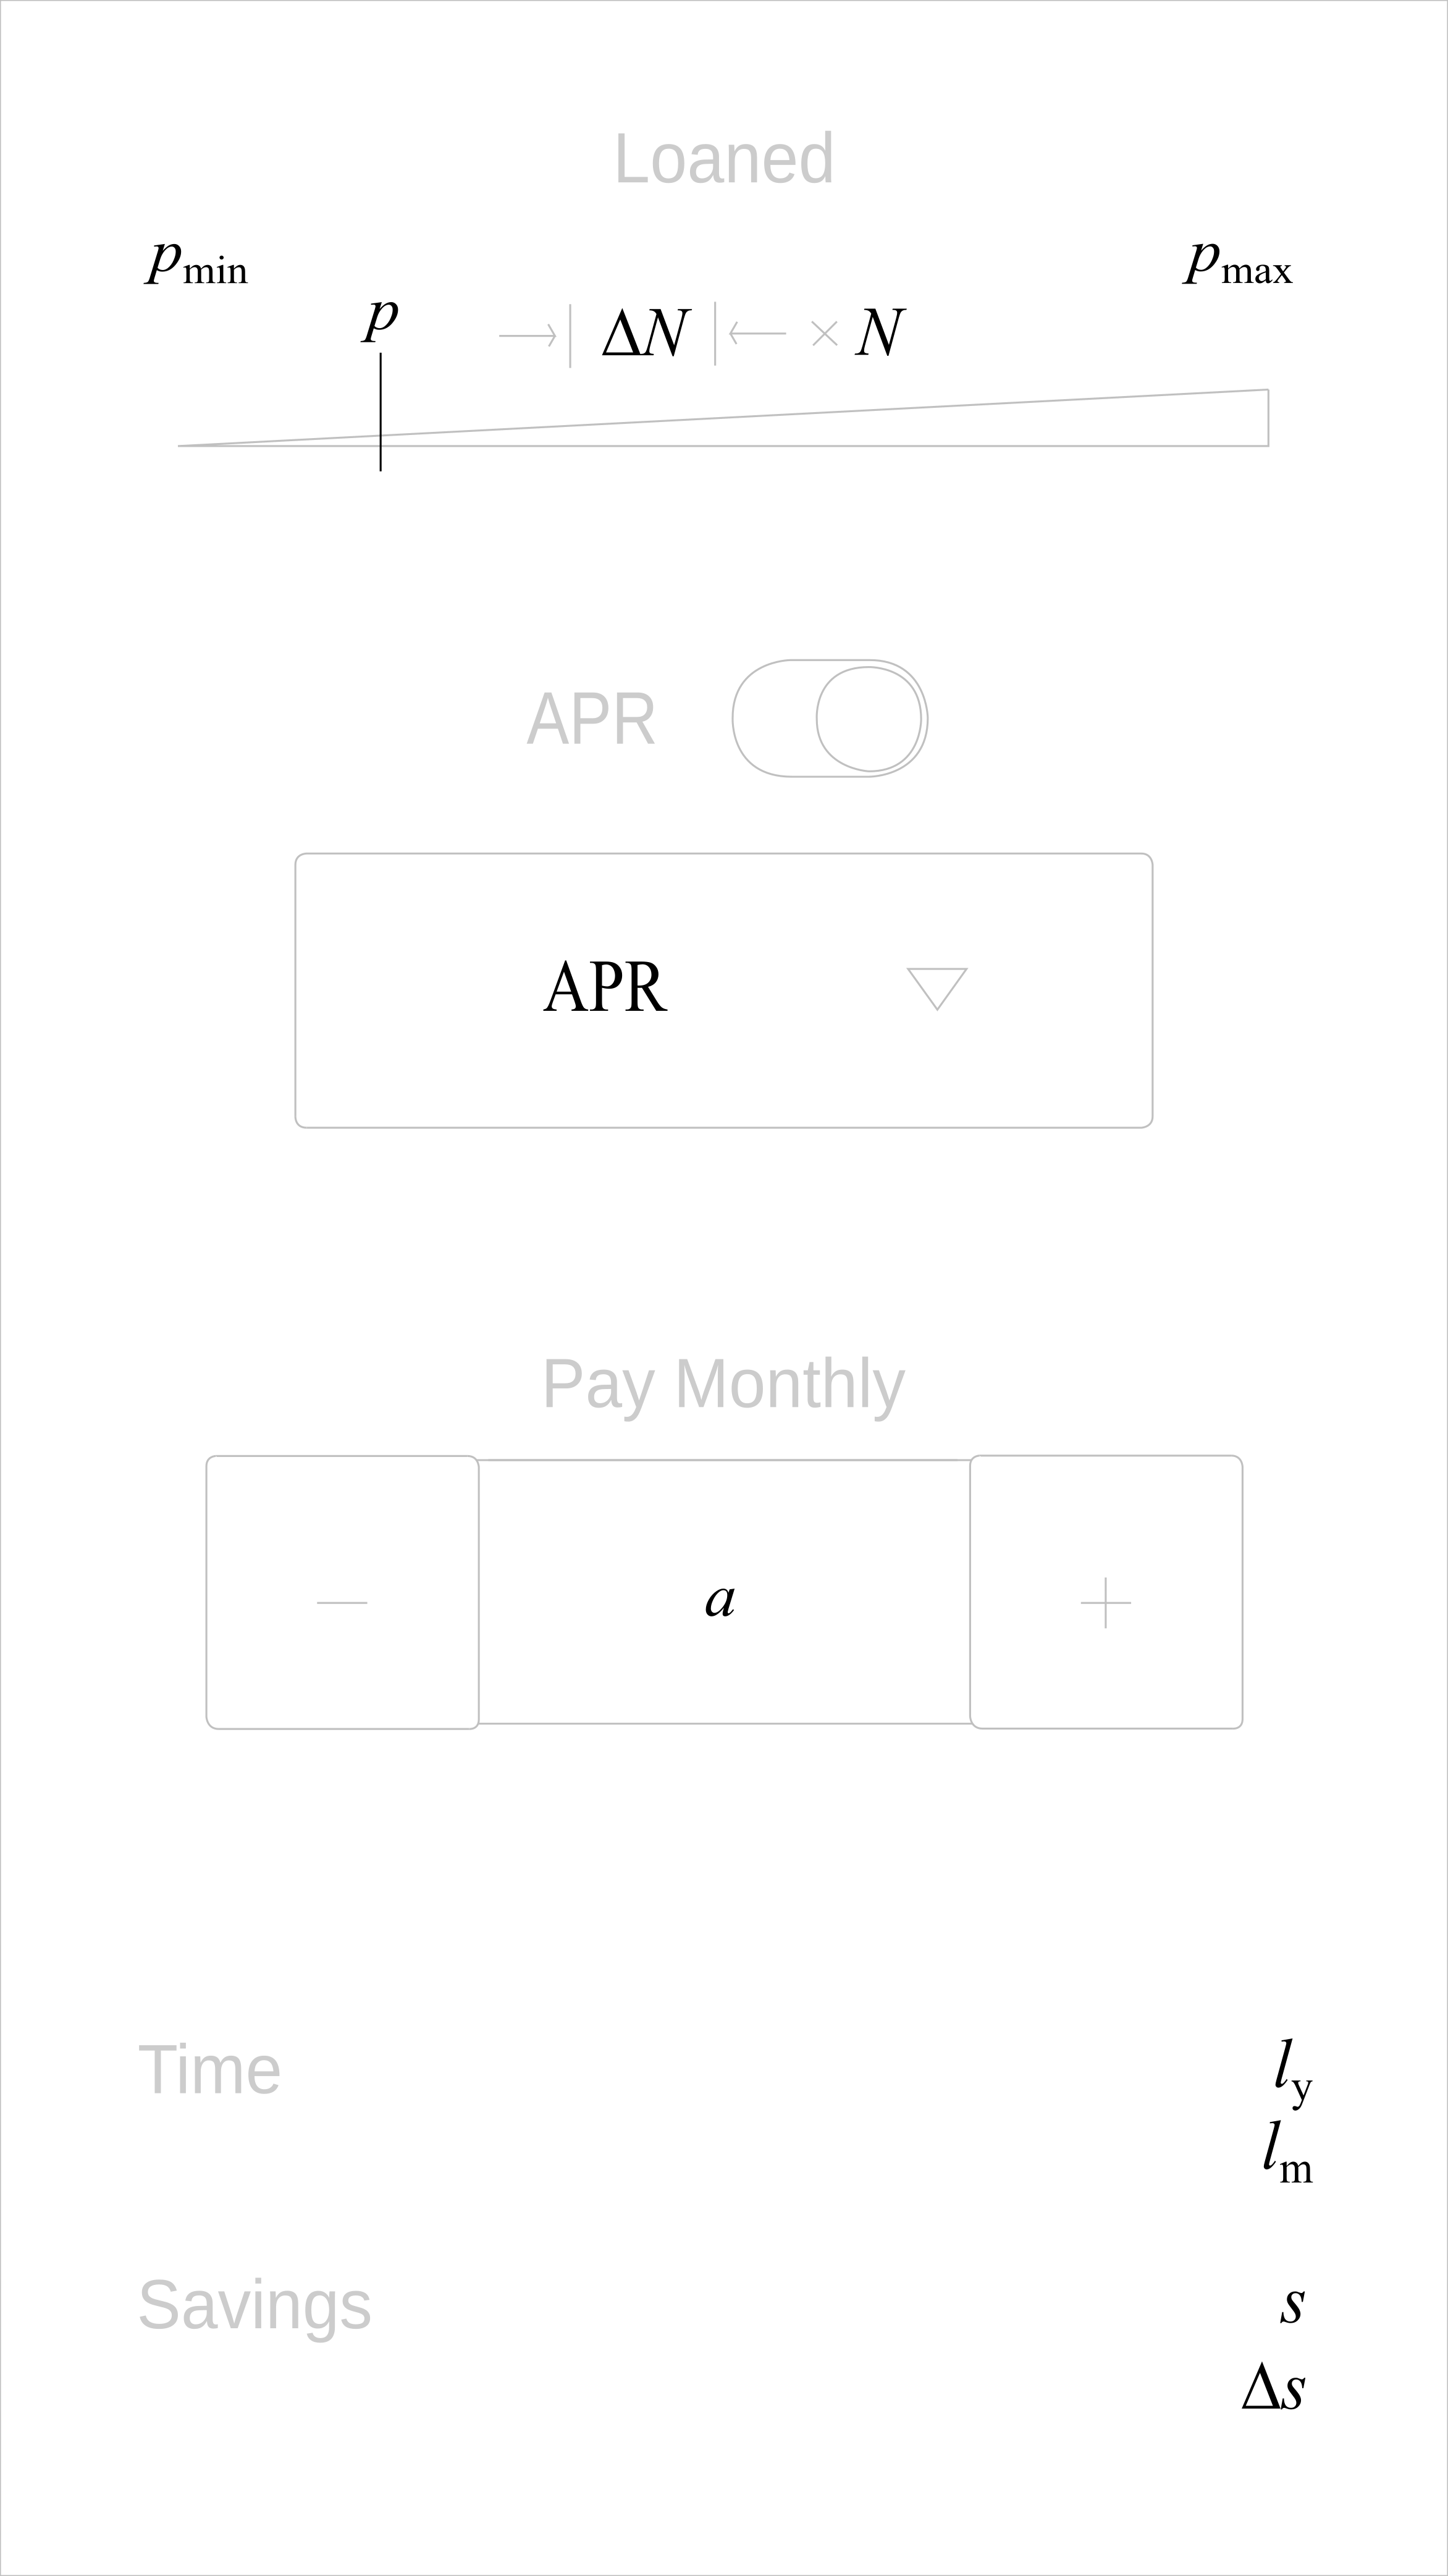
\includegraphics[height=4.6in]{main} & & 
	\qquad\ \ 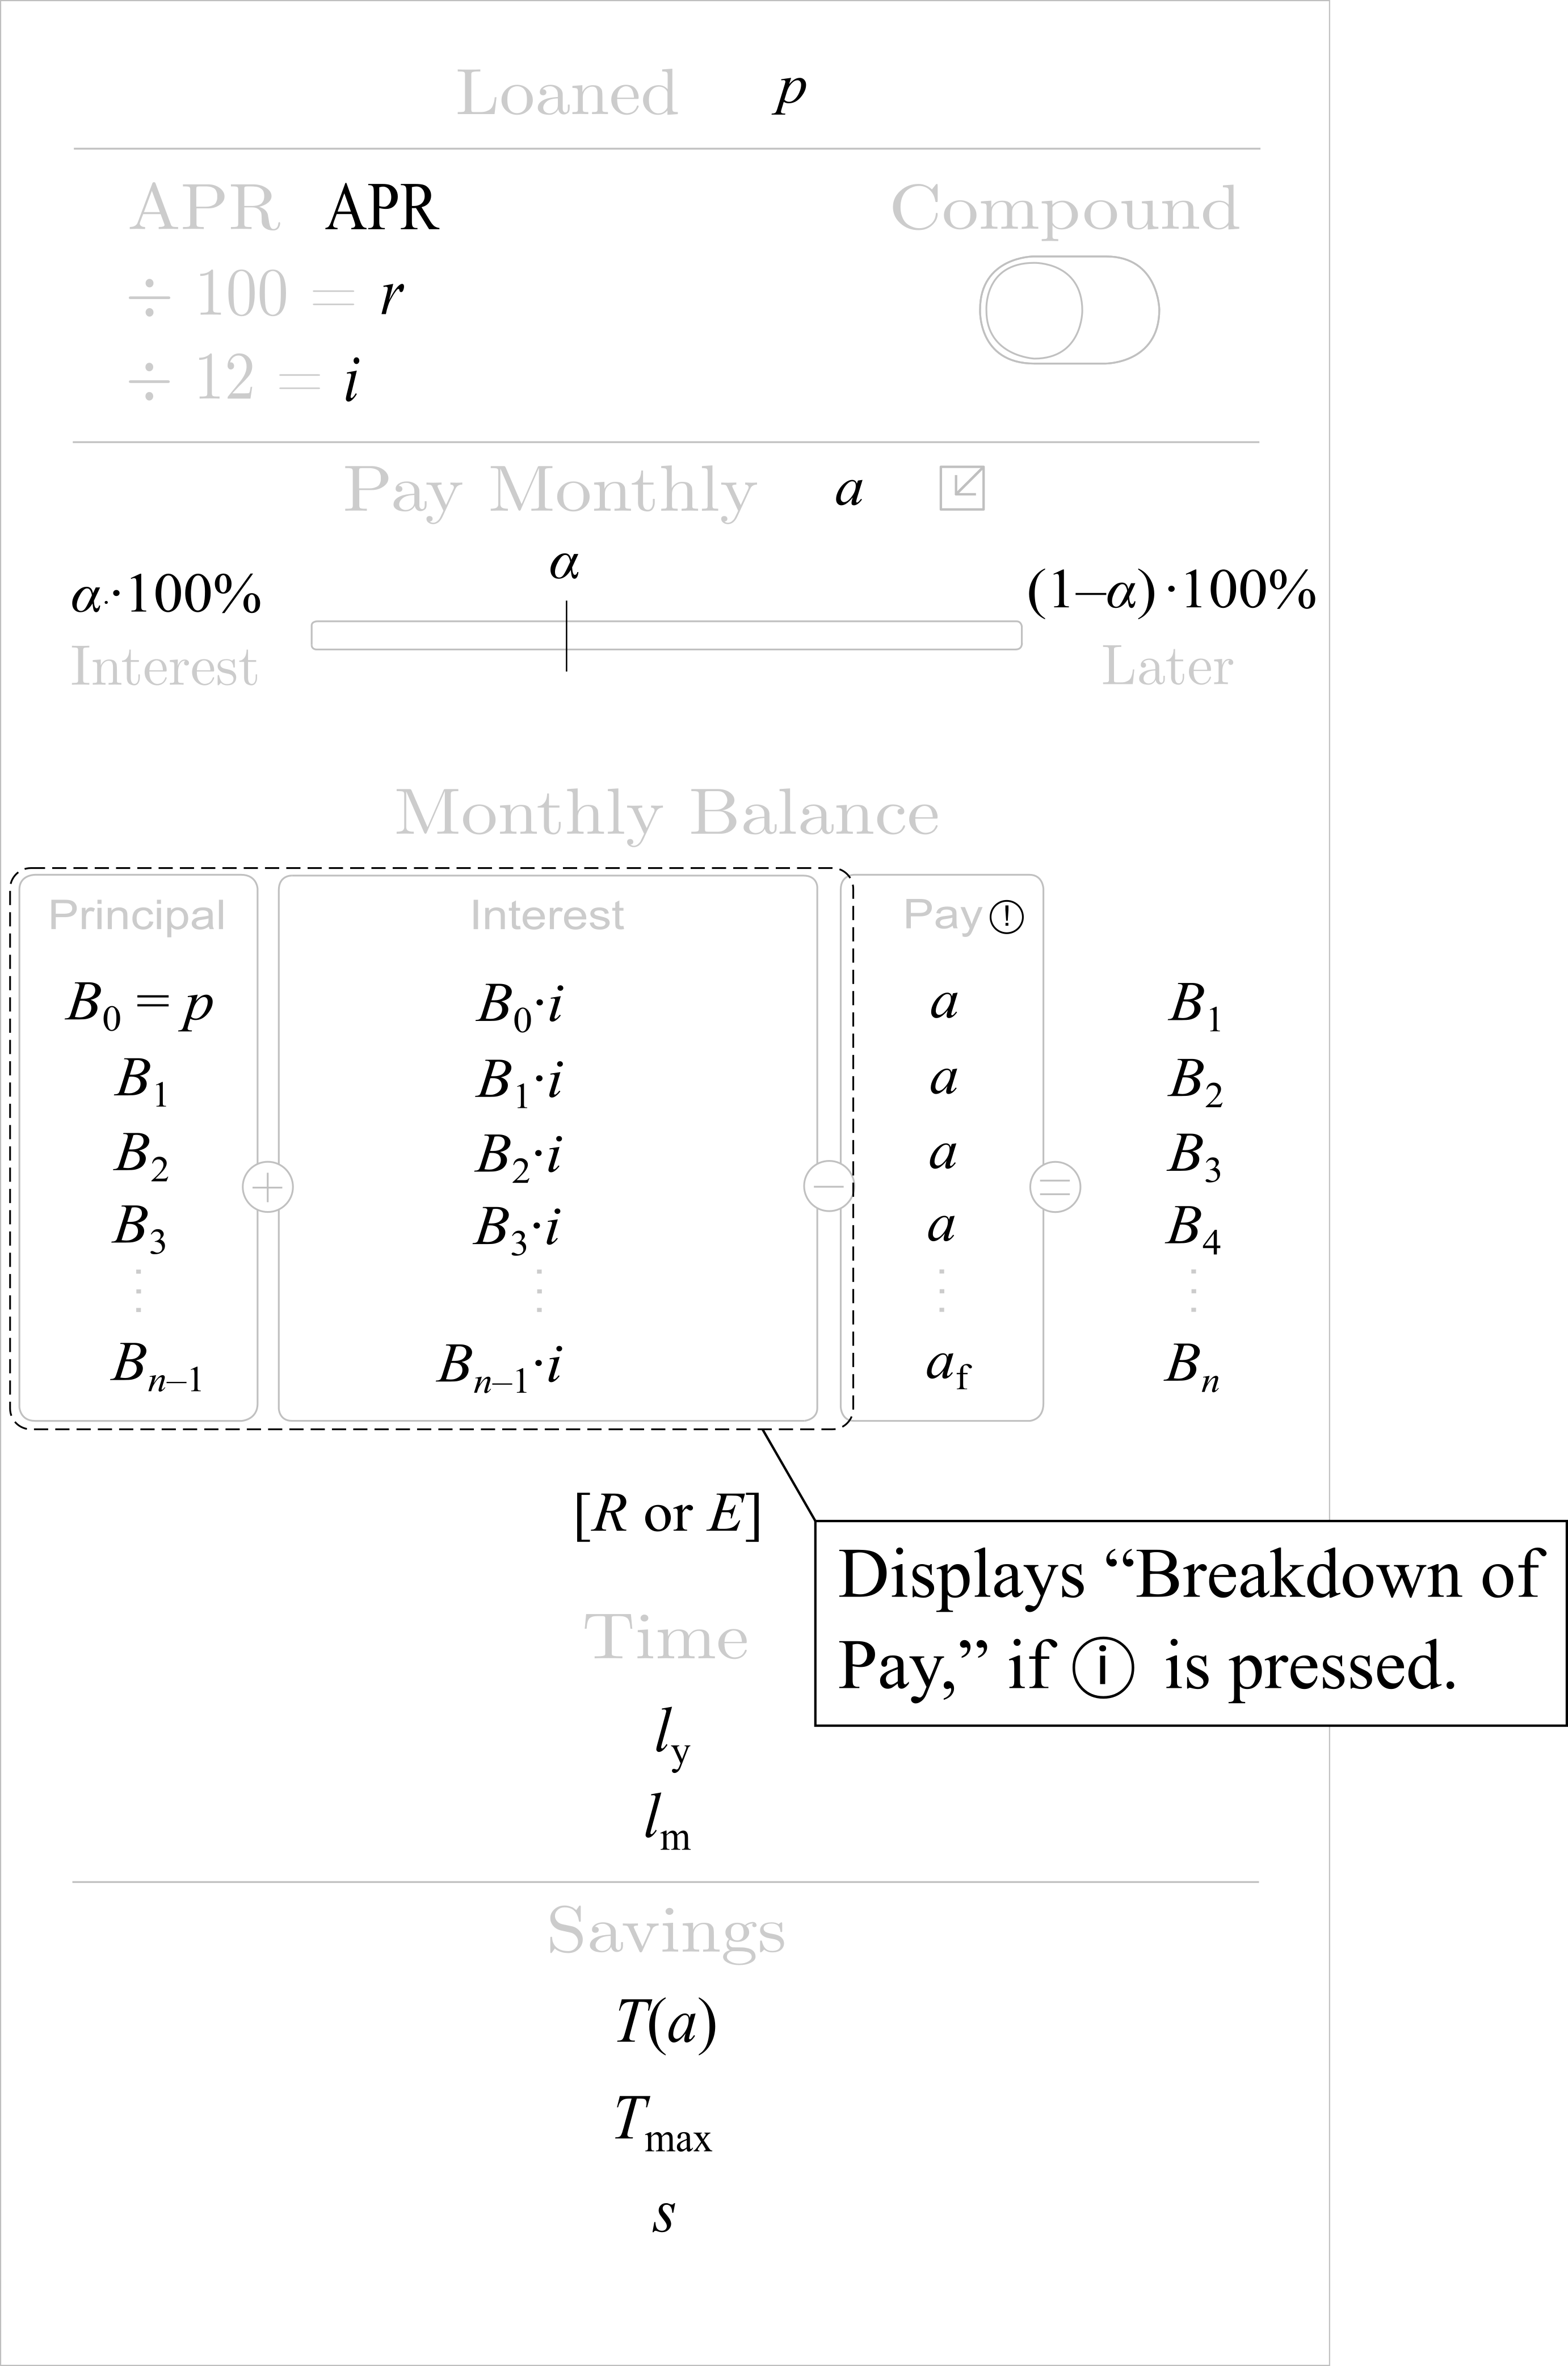
\includegraphics[height=4.6in]{math} \\[12pt] % \qquad is for spacing
	Not displayed: increment timers & \qquad\qquad & Caution: $a$ and $\alpha$ are different quantities. \\
	& & ``[\textit{R} or \textit{E}]'' means one or the other may be displayed. \\
	\end{tabular}
	\end{minipage}
	}
	\end{table}

	\newpage

\section{Terminology}

	Principal/initial balance (\$):
	$$\left\{\ p\ \middle|\ p\in\mathbb{W}\ \right\}$$
	Total increments (increments):\footnote{The researcher opted to capitalize variables that primarily involve totals.}
	$$\left\{\ N\ \middle|\ N\in\mathbb{N}\ \right\}$$
	Annual interest rate (/year):
	$$\left\{\ r\ \middle|\ r\in\frac{\mathbb{W}}{10,000}\ \right\}$$
	Monthly interest rate (/month):
	$$\left\{\ i\ \middle|\ i\in\mathbb{R}^{+}\cup\{0\}\ \right\}$$
	Monthly principal balance (\$):
	$$\left\{\ B\ \middle|\ B\in\frac{\mathbb{W}}{100},\ B\leq p\ \right\}$$
	Number of months (months):
	$$\left\{\ m\ \middle|\ m\in\mathbb{W}\ \right\}$$
	Monthly payment amount (\$):\footnote{See section~\ref{section2} for more information on $a_{\rm{min}}$, more specifically $a_{\rm{min_{\mathnormal{n}}}}$ and $a_{\rm{min_{120}}}$.}
	$$\left\{\ a\ \middle|\ a\in\frac{\mathbb{N}}{100},\ a\geq a_{\rm{min}}\ \right\}$$
	Proportion of interest that is paid (part):
	$$\left\{\ \alpha\ \middle|\ \alpha\in\frac{\mathbb{W}}{100},\ \alpha\leq 1\ \right\}$$
	Monthly outstanding interest (\$):
	$$\left\{\ O\ \middle|\ O\in\frac{\mathbb{W}}{100}\ \right\}$$
	Length of repayment (years):
	$$\left\{\ l_{\rm{y}}\ \middle|\ l_{\rm{y}}\in\mathbb{W}\ \right\}$$
	Length of repayment (months):
	$$\left\{\ l_{\rm{m}}\ \middle|\ l_{\rm{m}}\in\mathbb{N}\ \right\}$$
	Total payments (\$):
	$$\left\{\ T\ \middle|\ T\in\frac{\mathbb{N}}{100}\ \right\}$$
	Savings (\$):
	$$\left\{\ s\ \middle|\ s\in\frac{\mathbb{W}}{100}\ \right\}$$

	\newpage

\section{Formulae}\label{section2}

	Increment size (\$/increment):\footnote{See section 1 of ``Extra Insight into the iOS App'' for examples of all formulae.}
	$$\Delta N=\frac{p_{\rm{max}}-p_{\rm{min}}}{N},\mbox{ for }N\neq 0$$

	\setlength\parindent{0pt} Annual interest rate (/year):\footnote{Technically, $r=\mbox{APR}$, but some may not grasp the relationship between percents and decimals.}
	$$r=\mbox{APR(\%)}\div 100$$

	\setlength\parindent{0pt} Monthly interest rate (/month):\footnote{See section 2 of ``Extra Insight into the iOS App'' for more information on the compound interest rate.}
	\[
	\begin{array}{l l}
	i=\dfrac{r}{12} &\quad\mbox{if interest is \textit{not} compounded (default)}\\[12pt]
	i\approx\left(1+\dfrac{r}{365.25}\right)^{\frac{365.25}{12}}-1 &\quad\mbox{if interest is compounded}
	\end{array}
	\]

	\setlength\parindent{0pt} Monthly principal balance (\$):
	$$B_{m}=B_{m-1}-\big[a-\alpha\left(B_{m-1}\cdot i\right)\big]$$
	$$$$ % empty line to space out emphases
	$$\textcolor[rgb]{0.8,0.8,0.8}{B_{m}=B_{m-1}-\big[a\ -\emphasis{\ \alpha\left(B_{m-1}\cdot i\right)}{interest paid}\big]}$$
	$$\textcolor[rgb]{0.8,0.8,0.8}{B_{m}=B_{m-1}-\big[\emphasis{\ a-\alpha\left(B_{m-1}\cdot i\right)}{principal paid}\big]}$$

	\vspace{12pt} % add some padding above next sentence
	\setlength\parindent{0pt} Monthly outstanding interest (\$):
	$$O_{m}=O_{m-1}+\left(B_{m-1}\cdot i\right)-\alpha\left(B_{m-1}\cdot i\right)$$
	$$$$
	$$\textcolor[rgb]{0.8,0.8,0.8}{O_{m}=O_{m-1}\ +\emphasis{\ \left(B_{m-1}\cdot i\right)}{interest owed}-\ \alpha\left(B_{m-1}\cdot i\right)}$$ % \  for adding space between items that \colorbox compressed together
	$$\textcolor[rgb]{0.8,0.8,0.8}{O_{m}=O_{m-1}\ +\emphasis{\ \left(B_{m-1}\cdot i\right)-\ \alpha\left(B_{m-1}\cdot i\right)}{interest unpaid}}$$

	\vspace{12pt}
	\begin{remark}
	``Interest paid'' and ``interest owed,'' require an adjustment, however. Each of their terms may span more than two decimal places, and cents span only two, so round each quantity to the nearest two decimal places.
	\end{remark}

	\vspace{12pt}
	\setlength\parindent{0pt} Monthly principal balance (adjusted):
	$$B_{m}=B_{m-1}-\Big\{a-\big\lfloor{\alpha\left(B_{m-1}\cdot i\right)}\times\ 100\big\rceil\div 100\Big\}$$

	\setlength\parindent{0pt} Monthly outstanding interest (adjusted):
	$$O_{m}=O_{m-1}+\big\lfloor{\left(B_{m-1}\cdot i\right)\times 100}\big\rceil\div 100-\big\lfloor{\alpha\left(B_{m-1}\cdot i\right)\times 100}\big\rceil\div 100$$

	\begin{remark}
	For rounding $\alpha\left(B_{m-1}\cdot i\right)$, why not round $B_{m-1}\cdot i$ and then $\alpha\left(B_{m-1}\cdot i\right)$? This is because doing so would make computations less precise than by rounding once.
	\end{remark}

	\vspace{12pt}
	\setlength\parindent{0pt} Basic algorithm for computing the principal balance and outstanding interest:
	\begin{figure}[h] % ``h'' places algorithm directly beneath heading
	\centering
	\begin{minipage}{1.0\linewidth}
	\begin{algorithm}[H] % ``H'' stops algorithm from floating, capitalization matters and seems to differ between tables and figures
	\SetKwSty{texttt}
	\setstretch{1.25}	
	\texttt{set} $\quad B_{0}=p$ \;
	$\quad\quad\;\;\;\,O_{0}=0$ \;
	$\quad\quad\;\;\;\,m=1$\\
	\vspace{12pt}		
	\While{$\quad B_{m-1}-\Big\{a-\big\lfloor{\alpha\left(B_{m-1}\cdot i\right)\times 100}\big\rceil\div 100\Big\}>0\quad$}
	{
	$B_{m}=B_{m-1}-\Big\{a-\big\lfloor{\alpha\left(B_{m-1}\cdot i\right)\times 100}\big\rceil\div 100\Big\}$ \;
	$O_{m}=O_{m-1}+\big\lfloor{\left(B_{m-1}\cdot i\right)\times 100}\big\rceil\div 100-\big\lfloor{\alpha\left(B_{m-1}\cdot i\right)\times 100}\big\rceil\div 100$ \;
	$m=m+1$\\
	\vspace{6pt}
	}
	\vspace{12pt}
	\texttt{set} $\quad n=m$\\
	\texttt{set} $\quad a_{\rm{f}}=B_{n-1}+\big\lfloor{\left(B_{n-1}\cdot i\right)\times 100}\big\rceil\div 100\ \ +\emphasis{\ O_{n-1}}{paid now}$\;
	$\quad\quad\;\;\;\,B_{n}=B_{n-1}-\Big\{a_{\rm{f}}-\big\lfloor{\left(B_{n-1}\cdot i\right)\times 100}\big\rceil\div 100-O_{n-1}\Big\}\quad (=0)$\\[3pt]
	$\quad\quad\;\;\;\,(O_{n}=0)$
	\setstretch{1}
	\end{algorithm}
	\end{minipage}
	\end{figure}
	
	\begin{remark}
	Making outstanding interest due the final month is arbitrary. However, by doing so students may see the impact of interest on loans more clearly. Not only may final month's payment be higher, but also it may break equation~\ref{eq41}---as in \textit{break the bank}. 
	\end{remark}

	\vspace{12pt}
	\begin{remark}
	If one is programming the \texttt{while} loop in Swift, round $B_{m}$ and $O_{m}$ to the nearest two decimal places after each iteration of the loop. Otherwise, the values of $B_{m}$ and $O_{m}$ may drift by one cent or more over time. Simultaneously, inform Swift to round a quantity upward two places, if it has a hundredth remainder between, say, 0.499999 and 0.5 exclusive; otherwise, Swift will round downward. The researcher checked and rounded proportion of interest that is paid, interest owed, interest paid, $B_{m}$, $O_{m}$ and the absolute minimum monthly payment. He checked and rounded other quantities, as well, but doing so was not as crucial.
	\end{remark}

	% \newpage
	\vspace{12pt}
	Monthly Balance,
	\small
	\begin{align}\label{eq41}
	B_{0}\quad +\qquad\big\lfloor{\left(B_{0}\cdot i\right)\times 100}\big\rceil\div 100\quad -\quad a\quad =\quad B_{1}\nonumber\\
	B_{1}\quad +\qquad\big\lfloor{\left(B_{1}\cdot i\right)\times 100}\big\rceil\div 100\quad -\quad a\quad =\quad B_{2}\nonumber\\
	B_{2}\quad +\qquad\big\lfloor{\left(B_{2}\cdot i\right)\times 100}\big\rceil\div 100\quad -\quad a\quad =\quad B_{3}\nonumber\\
	B_{3}\quad +\qquad\big\lfloor{\left(B_{3}\cdot i\right)\times 100}\big\rceil\div 100\quad -\quad a\quad =\quad B_{4}\nonumber\\
	\vdots\qquad\qquad\qquad\qquad\qquad\qquad\ \ \vdots\qquad\quad\,\ \vdots\qquad\quad\ \ \ \:\vdots\nonumber\\
	B_{n-1}\quad +\quad\,\big\lfloor{\left(B_{n-1}\cdot i\right)\times 100}\big\rceil\div 100\ \ \ \;-\ \ \ a_{\rm{f}}\quad =\ \ \ \,B_{n}
	\end{align}
	
	Breakdown of Pay,
	\begin{align*}
	a-\big\lfloor{\alpha\left(B_{0}\cdot i\right)\times 100}\big\rceil\div 100\mbox{\ Prin.}&\quad +\quad \qquad\quad\ \ \ \big\lfloor{\alpha\left(B_{0}\cdot i\right)\times 100}\big\rceil\div 100\mbox{\ Int.}&\, =\quad a&\\
	a-\big\lfloor{\alpha\left(B_{1}\cdot i\right)\times 100}\big\rceil\div 100\mbox{\ Prin.}&\quad +\quad \qquad\quad\ \ \ \big\lfloor{\alpha\left(B_{1}\cdot i\right)\times 100}\big\rceil\div 100\mbox{\ Int.}&\, =\quad a&\\
	a-\big\lfloor{\alpha\left(B_{2}\cdot i\right)\times 100}\big\rceil\div 100\mbox{\ Prin.}&\quad +\quad \qquad\quad\ \ \ \big\lfloor{\alpha\left(B_{2}\cdot i\right)\times 100}\big\rceil\div 100\mbox{\ Int.}&\, =\quad a&\\
	a-\big\lfloor{\alpha\left(B_{3}\cdot i\right)\times 100}\big\rceil\div 100\mbox{\ Prin.}&\quad +\quad \qquad\quad\ \ \ \big\lfloor{\alpha\left(B_{3}\cdot i\right)\times 100}\big\rceil\div 100\mbox{\ Int.}&\, =\quad a&\\
	&&\vdots&\\
	B_{n-1}\mbox{\ Prin.}&\quad +\quad\ \:\:\big\lfloor{\left(B_{n-1}\cdot i\right)\times 100}\big\rceil\div 100+O_{n-1}\mbox{\ Int.}& =\,\ \ \,a_{\rm{f}}&
	\end{align*}
	\normalsize

	\setlength\parindent{0pt} Length of repayment (years):
	$$l_{\rm{y}}=\bigg\lfloor{\frac{n}{12}}\bigg\rfloor$$

	\setlength\parindent{0pt} Length of repayment (months):
	$$l_{\rm{m}}=n-12\cdot l_{\rm{y}}$$

	\setlength\parindent{0pt} Special cases of algorithm:\footnote{For simplicity, let us assume the refund is sent, or extra pay is made, immediately thereafter.}
	\begin{figure}[h]
	\centering
	\begin{minipage}{1.0\linewidth}
	\begin{algorithm}[H]
	\SetKwSty{texttt}
	\setstretch{1.25}	
	\If{$\quad n=1\quad$}{
	\uIf{$\quad a-a_{\rm{f}}>0\quad$}{
	$R=a-a_{\rm{f}}$ \;
	\texttt{display}\quad ``Refunded \$\textbf{[}$R$\textbf{]}''\\
	\vspace{6pt}
	}
	\ElseIf{$\quad a-a_{\rm{f}}<0\quad$}{
	$E=\left|a-a_{\rm{f}}\right|$ \;
	\texttt{display}\quad ``Pay Extra \$\textbf{[}$E$\textbf{]}''\\
	\vspace{6pt}
	}
	\vspace{6pt}
	}
	\setstretch{1}
	\end{algorithm}
	\end{minipage}
	\end{figure}

	% \newpage
	\begin{remark}
	Be mindful of the differences between $\lfloor{\ }\rceil$, $\lfloor{\ }\rfloor$ and $\left|\;\ \right|$. The former brackets correspond to the nearest integer (i.e., \texttt{nint}) function, middle ones to the nearest lowest integer (i.e., \texttt{floor}) function, and latter the absolute value (i.e., \texttt{abs}) function.
	\end{remark}

	% \newpage
	\vspace{12pt}
	\setlength\parindent{0pt} Absolute minimum monthly payment (\$):
	$$a_{\rm{min_{\mathnormal{n}}}}=\big\lfloor{\alpha\left(p\cdot i\right)\times 100}\big\rceil\div 100+0.01$$
	$$$$
	$$a_{\rm{min_{\mathnormal{n}}}}=\quad\quad\quad\emphasis{\ \big\lfloor{\alpha\left(p\cdot i\right)\times 100}\big\rceil\div 100}{applied to interest}\quad\quad\quad+\ \emphasis{\ 0.01}{applied to principal}$$

	\vspace{12pt}
	\setlength\parindent{0pt} Ten-year minimum monthly payment (\$):\footnote{See section 3 of ``Extra Insight into the iOS App'' for more information on the ten-year payment.}
	\newcommand{\base}{\left(1+\alpha\cdot i\right)}
	\small
	\[
	a_{\rm{min_{120}}}=
	\left\{
	\begin{array}{l l}
	\\[-6pt] % additional padding for bracket
	\left\lceil{\dfrac{p}{120}\times 100}\right\rceil\div 100&\quad\mbox{if } i>0 \mbox{ and }\alpha=0\\[18pt] % spacing out some more
	\left\lceil{\dfrac{p}{120}\times 100}\right\rceil\div 100&\quad\mbox{if } i=0\\[12pt]
	\left\lceil{\dfrac{\alpha\left(p\cdot i\right)\base^{120}}{\base^{120}-1}\times 100}\right\rceil\div 100,\mbox{ for }\alpha\cdot i\neq 0 &\quad\mbox{if } i>0\mbox{ and }0<\alpha\leq1
	\\[18pt] % additional padding for bracket
	\end{array}
	\right. 
	\]
	
	\normalsize
	\begin{remark}
	Ten-year minimum monthly payment is for repaying student loans within ten years, \textit{not} for repaying student loans for at least ten years.
	\end{remark}

	\vspace{12pt}
	\setlength\parindent{0pt} Total payments (\$):
	$$T(a)=(n-1)a+B_{n-1}+\big\lfloor{\left(B_{n-1}\cdot i\right)\times 100}\big\rceil\div 100+O_{n-1}$$
	$$T_{\rm{max}}=(n-1)a_{\rm{min}}+B_{n-1}+\big\lfloor{\left(B_{n-1}\cdot i\right)\times 100}\big\rceil\div 100+O_{n-1}$$

	\vspace{12pt}
	\setlength\parindent{0pt} Savings (\$):
	$$s=T_{\rm{max}}-T(a)$$

	\vspace{12pt}
	\begin{remark}
	Each total payment still accounts for $\alpha$. As $\alpha$ increases, $n$ increases and $O_{n-1}$ decreases; this is because every month less money is applied to principal and more is applied to interest. As $\alpha$ decreases, the opposite effect occurs because more money is applied to principal and less to interest.
	\end{remark}

	\vspace{12pt}
	\setlength\parindent{0pt} Change in savings (\$):
	$$s_{1}=T_{\rm{max}}-T(a_{1}),\mbox{ where }a_{1}\geq a_{\rm{min}}$$
	$$s_{2}=T_{\rm{max}}-T(a_{2}),\mbox{ where }a_{2}\geq a_{\rm{min}}$$
	$$\Delta s=\left|s_{2}-s_{1}\right|$$

	\vspace{12pt}
	\begin{remark}
	The direction of change will be indicated with an up or down arrow.
	\end{remark}

\end{document}